As described above, we plan a suite of comprehensive simulations of
XRBs and SNe Ia (both the sub-Ch and WDWD models) using our
codes \maestro\ and \castro.  All the problems we
describe are inherently three-dimensional, requiring large resources.
Our codes are running on titan today, and they perform and scale
well.  The starting point for all the simulations proposed are in
place.  We are ready to run.

The calculations we describe in further detail here are INCITE--class
for two reasons.  First, as is often the case in astrophysics, we can
never capture all the length-scales that come into play in these
stellar explosions, for example, the turbulent dissipation scale in
the convective regions is often quite below our grid resolution.  As a
result, we need to push to higher-and-higher resolution to assess
whether our results are converged.  This high resolution demands a lot
of computational resources---the type that only INCITE can provide.
Second, the temporal scales we need to model are equally impressive.
For the XRB simulations, we would like to model a second of evolution.
At our current resolution (6~cm), we would need over a million
timesteps (and that is with the large efficiency gain we get through
the low Mach model).  Since there is no parallel-in-time equivalent to
domain decomposition, we need to run a big problem for long amounts of
time on the machine---again, a feat only possible through INCITE.
Finally, we want to push the realism of the physics, in particular,
our reaction networks.  This will only be feasible by offloading some
of the reaction expense to the GPUs.

The basic motivation for our science problems was given in the
previous section.  Here we begin by discussing the milestones we hope
to achieve in each year and then we give specific details about the
number and size of the simulations we plan to run.  We note that because
we have preliminary calculations of each of the problems we propose to
run, we can base our time requests on existing simulations from titan
(here Mh = mega-hours).  Also, there is a pattern to our milestones:
one milestone for each of the major topics per year (XRBs, sub-Ch,
WDWD), the utilization of the GPU-enhanced reaction network becomes the norm in year 2,
and the application of new features (rotation and sub-grid models in
\maestro) and the transfer capability from \maestro\ to \castro.
The \maestro\ calculations make up most of the time request in year 1, but
by year 3, that proposed \castro\ and \maestro\ calculations reach parity.

\begin{tightitem}
\item {\bf Year 1: 80 Mh total }
%
\begin{tightitem}
\item {\em Full star, high-resolution \maestro\ models of convection
  in sub-Ch WDs}: Many simulations will be performed, with
  various initial models.  Our experience shows that a moderately-high
  resolution simulation requires about 0.5~Mh and we imagine 20 runs.
  We would like to do 5 higher resolution runs, which we budget at 4~Mh
  each.  {\em total: 30 Mh}

\item {\em Large domain \maestro\ XRB convection models}: Our current
  3D XRB simulation (in a domain 15~m wide) will require about 2 Mh.
  On titan, we would like to run something that is 2$\times$ wider in
  the transverse directions, bring the cost of a single simulation to
  8 Mh.  We will do two of these in year 1 (with different initial
  models), as well as a number of smaller exploratory calculations to
  test the effects of bigger reaction networks (with GPUs).  We budget 
  4 Mh for the exploratory
  calculations).  {\em total: 20~Mh}

\item {\em \castro\ multi-orbit WDWD inspiral and merger}: We want
  to follow up to 5 orbits of the white dwarf pair to capture the
  tidal disruption and first contact.  Three models will be done
  with various WD masses.  Our estimates are 10~Mh per simulation
  (based on our initial runs on titan).  {\em total: 30~Mh}
\end{tightitem}
%  
\item {\bf Year 2: 111 Mh total}
%
\begin{tightitem}
\item {\em \maestro\ sub-Chandra SNe Ia models with large reaction
  networks}: These calculations will be the follow-on to year 1, using
  more detailed initial models and larger (20-40 isotope) reaction
  networks.  We expect that with the GPUs handling the reactions that
  we will see only a modest increase in cost despite the much larger
  network.  We budget 2 Mh per simulation, with the goal of doing 10
  simulations.  {\em total: 20~Mh}

\item {\em \maestro\ XRB convection models with large reaction networks}:
  This will be the follow-on to year 1.  Again, we hope to push the
  size of the domain and increase the size of the network.  Since we 
  are already using a moderate network, we expect that the GPUs
  can offset the size of the network.  If we double the width of
  the domain again, we put the cost of a simulation at 32 Mh.  We 
  will do a single simulation at this scale, plus two more
  at the size from year 1. {\em total: 40~Mh}

\item {\em \castro\ WDWD models with nuclear physics}:
  These calculations will pick up where year 1 left off.  We will now 
  model the details of the merger event itself, with a reaction network
  to assess the potential for prompt ignition.  The number of cells 
  in the calculation is expected to increase with the complexity of 
  the flow (through AMR), so we need to scale the time requirements
  accordingly.  We budget 25~Mh for each calculation, and wish to 
  perform 2 (different initial conditions). {\em total: 50~Mh}

\item {\em Exploratory \maestro\ URCA calculations}:  As discussed
  above, this is a direct application of the methodology we used
  for the Chandra ignition calculations during our current award.
  We will budget 1 Mh for a single 3D calculation of the URCA
  convection.  {\em total: 1~Mh}
\end{tightitem}
%
\item {\bf Year 3: 122~Mh total}
%
\begin{tightitem}
\item {\em \maestro\ to \castro\ models of sub-Ch SNe Ia}: 
   We will use one of our existing \maestro\ sub-Ch models from year 2
   to initialize a \castro\ simulation.  We have made this
   transfer before with the Chandra models.  Our estimate for
   the time required for this simulation is based on pure \castro\
   models of sub-Ch explosions, and we place it at 10 Mh.  {\em total: 10~Mh}

\item {\em More realistic \maestro\ sub-Ch SNe Ia models}: These
  calculations will improve upon those from year~2.  We will use more
  realistic initial models from the MESA stellar evolution code and we
  will perform some simulations with rotation.  The rotation
  simulations rely on expected development in \maestro.  The overall
  cost of the calculations should be comparable to the year 2 models,
  and we budget 2 Mh per simulation and hope to repeat the same 10
  models from year 2.  {\em total: 20~Mh}

\item {\em Sensitivity study of XRB simulations (\maestro)}:
   We will perform several more XRB convection models with different
   (and more realistic) initial models.  We budget these as in year 1
   at 8~Mh, and hope to do 4 calculations.  {\em total: 32~Mh}
   
\item {\em Large-scale XRB burning model with sub-grid burning}:
  This calculation relies on the development of a subgrid model
  using the simulations from years 1 and 2 as a basis.  The time estimate
  depends on how much we are allowed to relax the resolution requirements,
  which is unknown at this time.  We will be in a better position to
  estimate the time in mid-year 2, but we pick 10~Mh as a representative
  estimate for a big 3D convection problem with \maestro.  {\em total: 10~Mh}

\item {\em \castro\ WDWD models with realistic initial conditions}:
  These calculations will continue those from year 2, but we will incorporate
  models from stellar evolution codes to give us a more realistic 
  composition and structure.  In particular, we will explore some models
  with a think He layer on the surface.  The cost should be the same
  as in year 2.  {\em total: 50~Mh}

\end{tightitem}
%
\end{tightitem}

\begin{figure}[t]
\centering
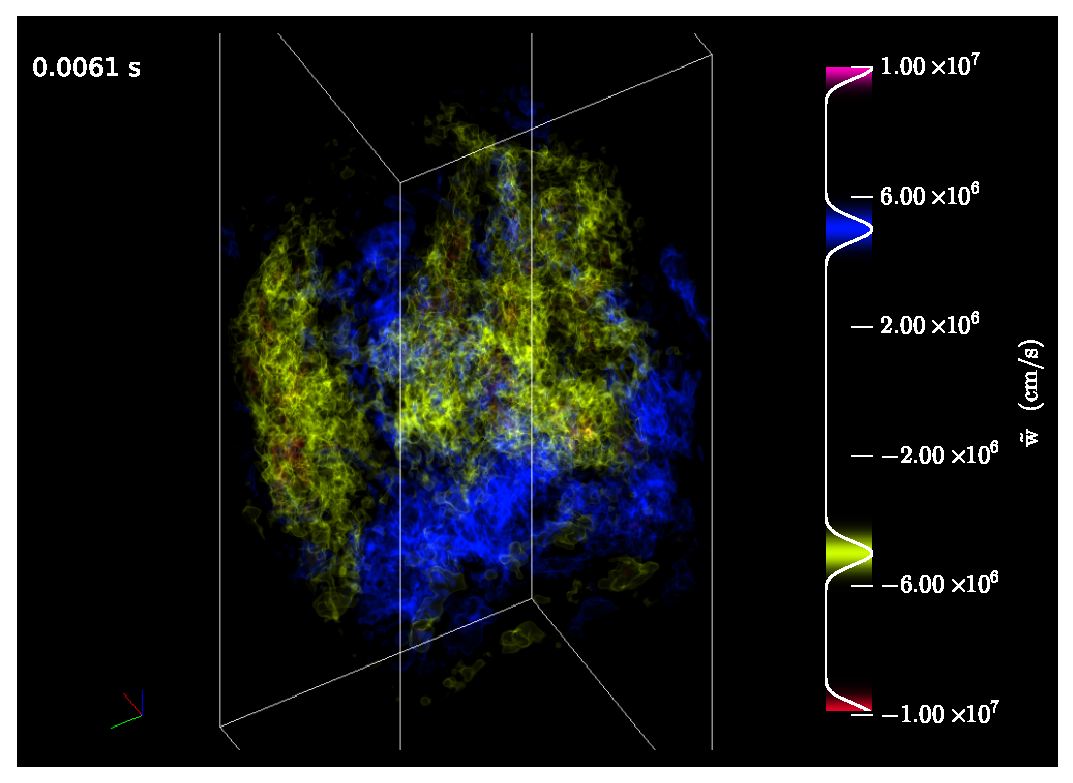
\includegraphics[width=0.42\linewidth]{xrb_vol_vz}
\hspace{0.25em}
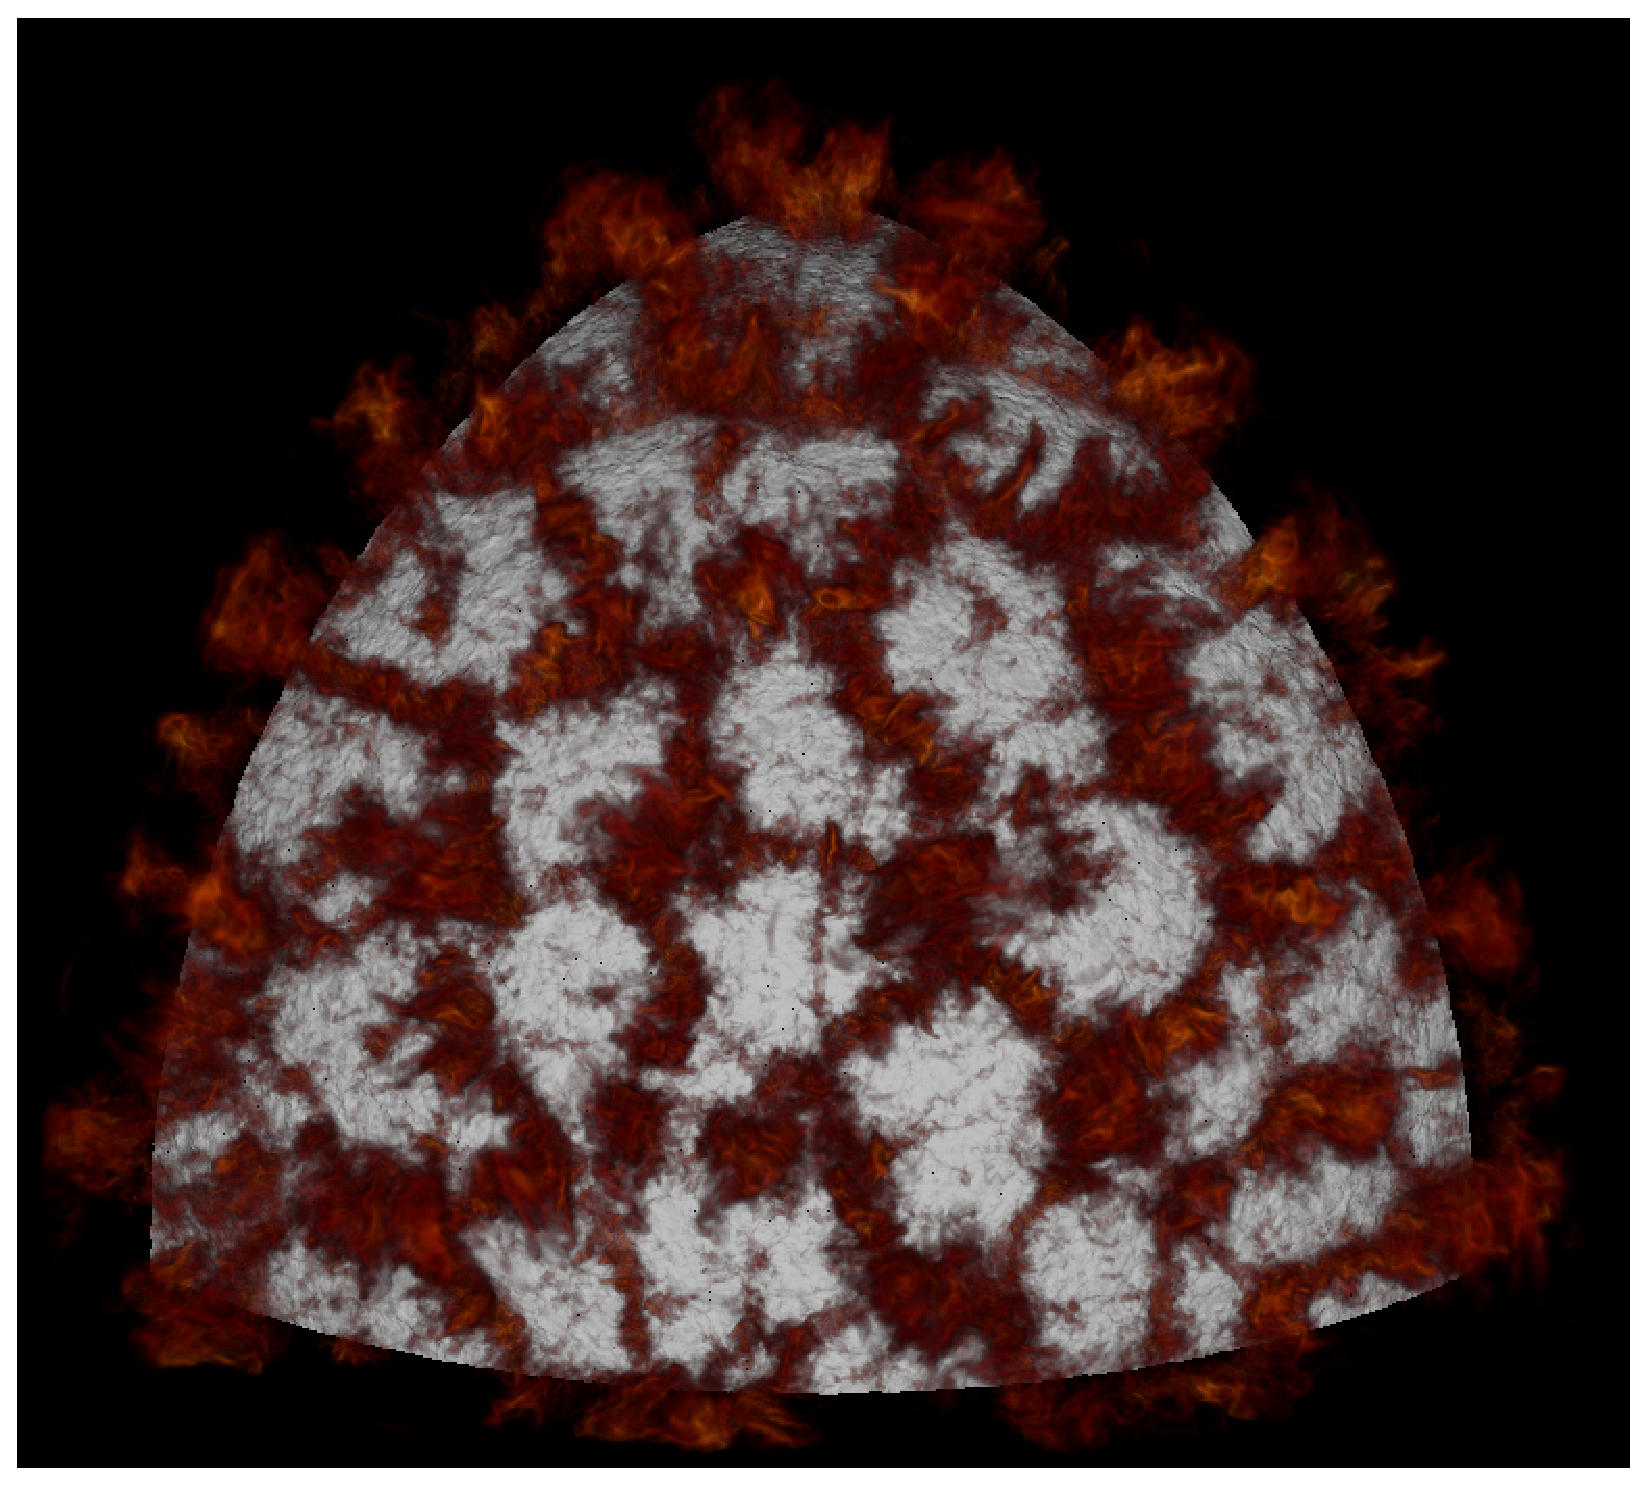
\includegraphics[width=0.32\linewidth]{ConvPlumes} \\[0.1em]
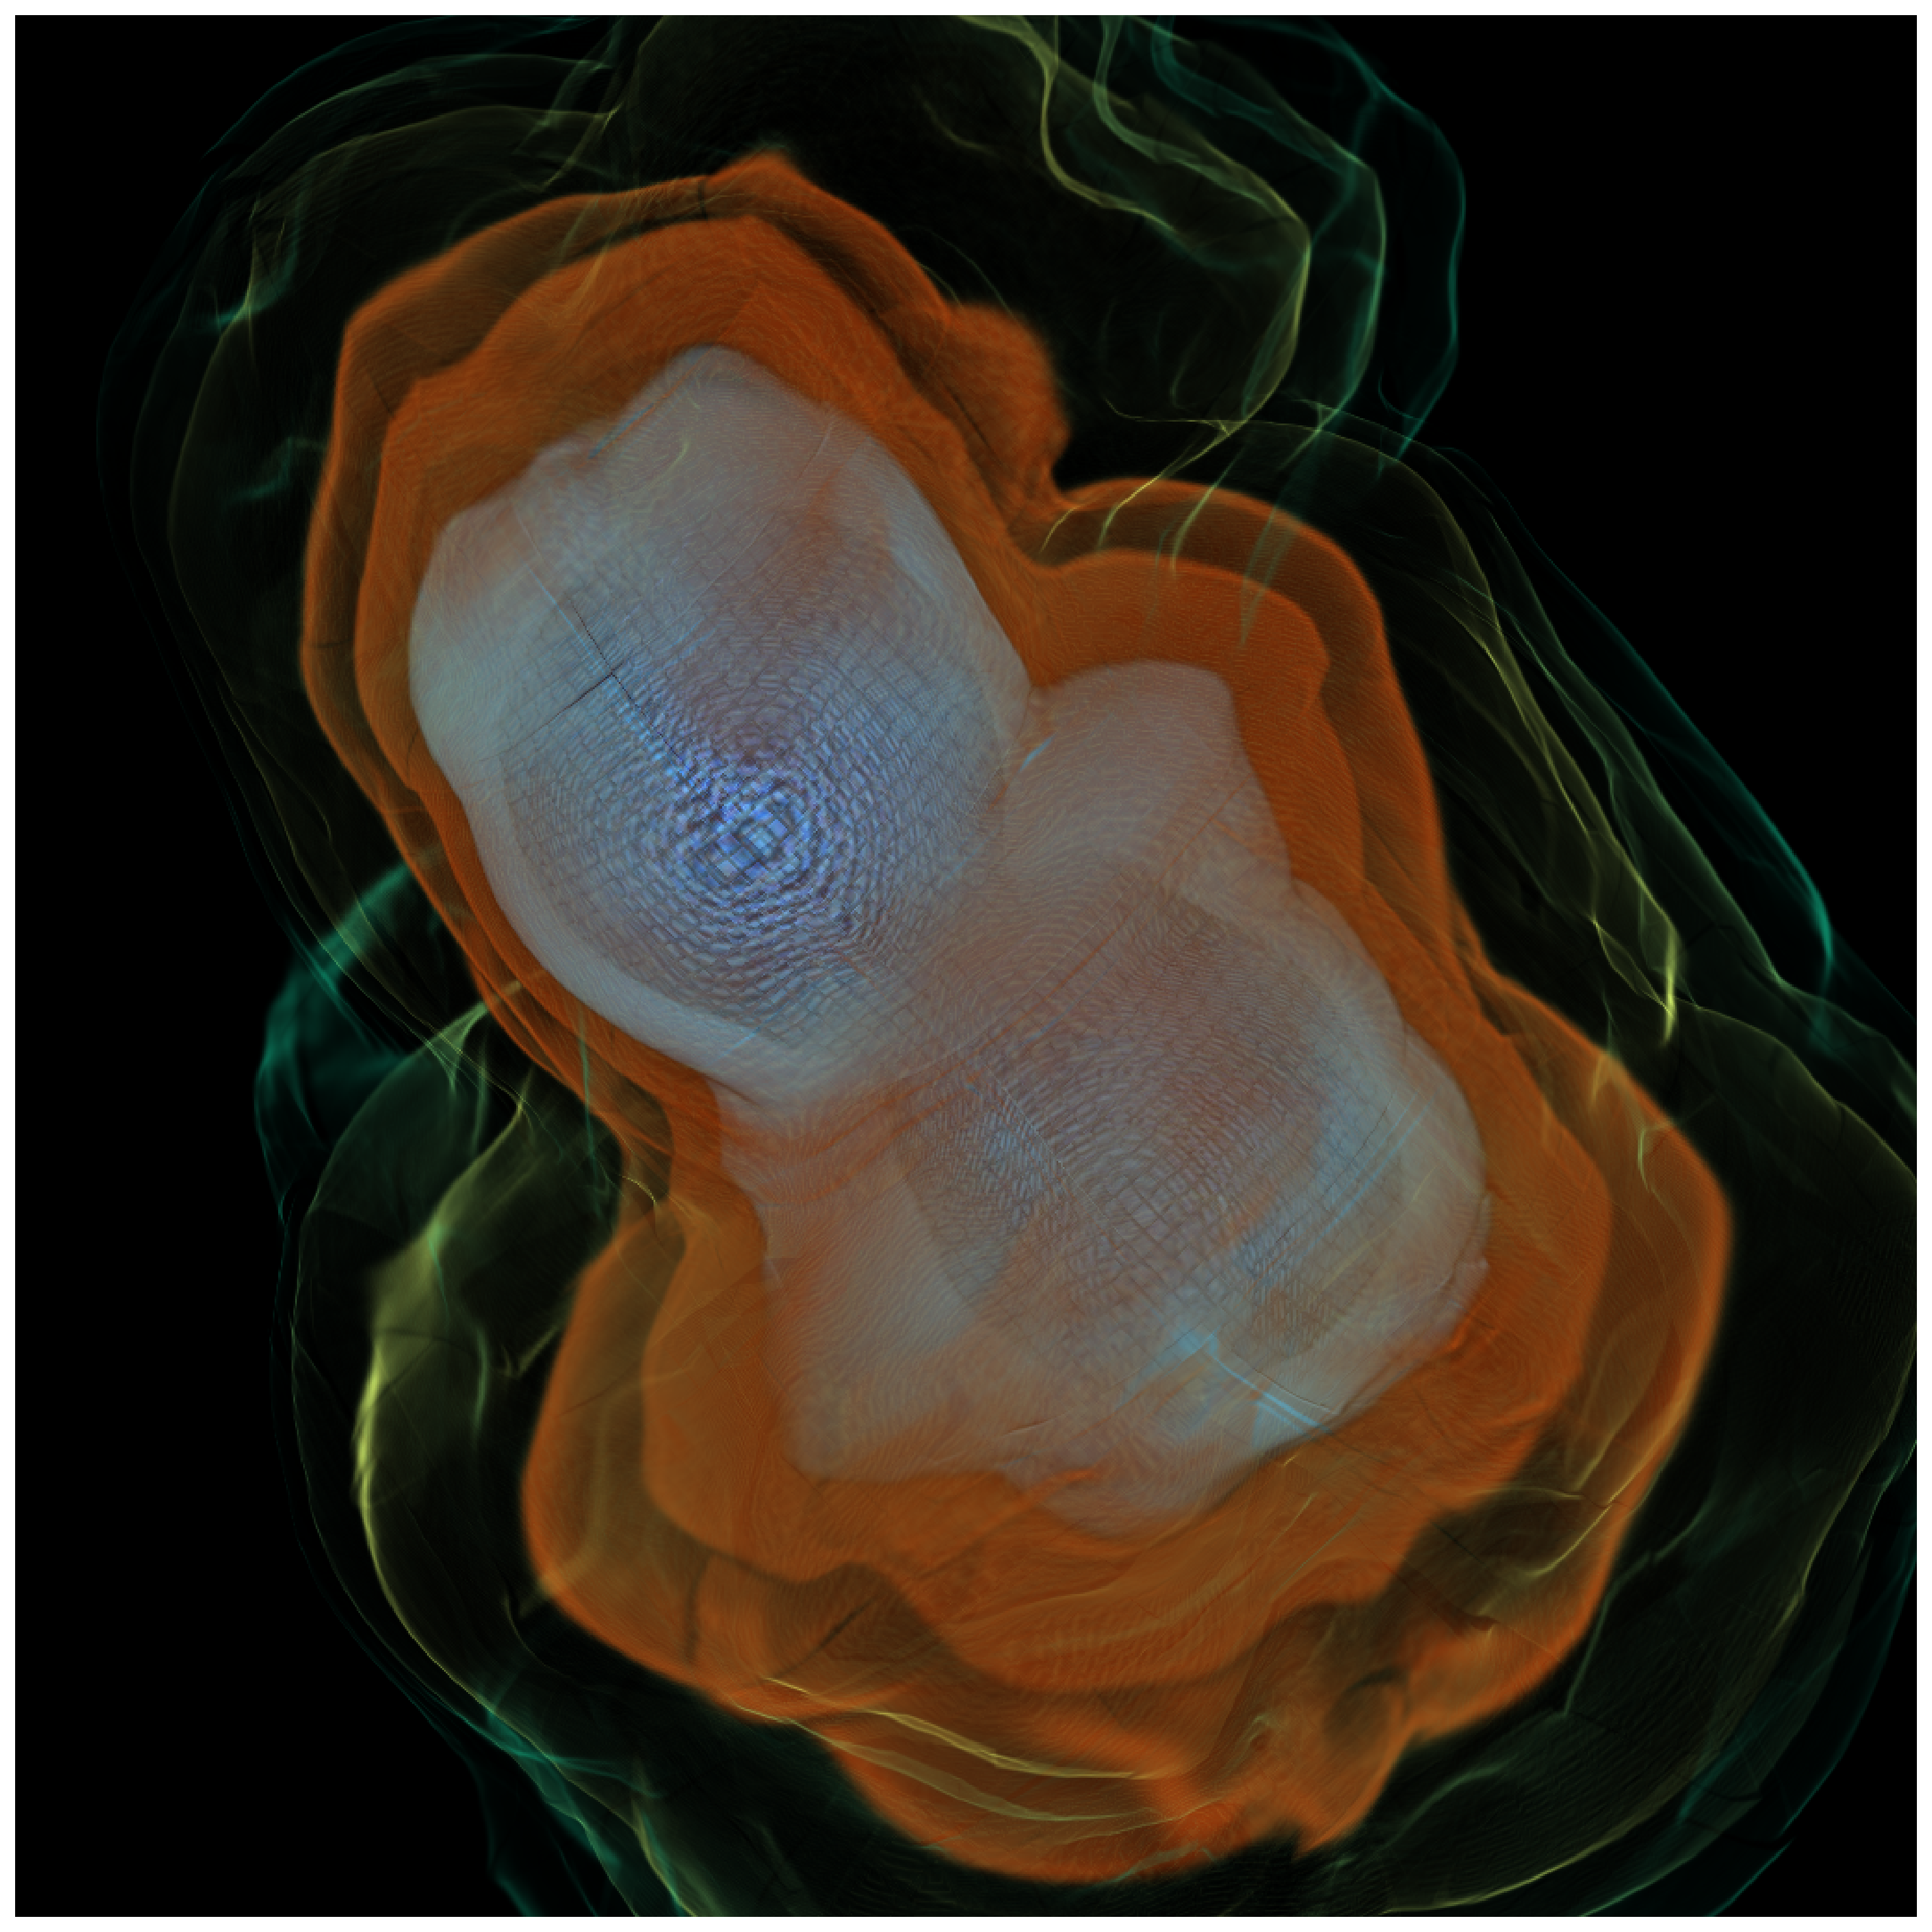
\includegraphics[width=0.3\linewidth]{generic3plt00180}\hspace{0.5em}
\begin{minipage}[b]{0.44\linewidth}
\caption{\label{fig:current-runs} (top left) Vertical velocity showing the
  convective structure in a \maestro\ XRB calculation.  (top right)
  Convective plumes in a \maestro\ sub-Ch calculation.  (left)
  Snapshot of a \castro\ simulation of the merger of two white dwarfs,
  with 0.90 and 0.81 solar masses. The contours represent density
  levels. The star on the upper left is disrupting and accreting onto
  the other star.}
\end{minipage}
\end{figure}


{\bf XRB simulations}:  Figure~\ref{fig:current-runs} shows
a snapshot from a current \maestro\ XRB simulation.
Our
2D study~\cite{XRB2} showed us that in order to resolve the 
nuclear burning, we needed to use a model with 6 cm resolution.
The current 3D simulation is done on a 256$\times$256$\times$768
grid.  At this resolution, we achieve timesteps of about $0.3~\mathrm{\mu s}$,
and this running this calculation to 0.1~s would require about 2 Mh on titan.

There two are primary goals for the XRB simulations.  First, we want to run
larger domains.  When the domain is small, the boundaries confine the convective
rolls, and an artificial flow is setup.  We want the width of the domain to be
several times larger than the scale height ($\sim 10$~m).  Keeping the
resolution fixed at 6~cm, we will perform simulations in 30~m and 60~m wide
domains.  These will give a clear picture of the dynamics of the convection
and allow us to answer the questions posed in the previous section:
how does the convection alter the nucleosynthesis? and are ashes brought
up to the surface where they can change the observables?

Secondly, we want to enable even larger domains by relaxing the
resolution requirements.  Using the results from years 1 and 2, we
will work on developing a sub-grid burning model that can be used to
capture the dynamics of the convection at coarser resolution.  We will
then push the domain sizes to 100s~m.  At this point, we can find ourselves
with burned regions in one part of the domain and unburned in others.  
Describing these different vertical structures is not currently possible
in \maestro\ (the different temperatures and composition result in different
hydrostatic structures, and \maestro\ is built on modeling the flow superposed
on a hydrostatic background).  Nevertheless, allowing for lateral gradients is 
in the plans for \maestro's development, and we hope to be in the position
to capture this new dynamics by year 3.

For the year 1 and 2 calculations, the resolved nuclear burning will require
us to use accurate reaction networks.  At the moment, we use a 10-isotope
network that captures the hot-CNO H burning, 3-$\alpha$ He burning, and some
links to heavier elements and the rp-process.  Our current study showed that
approximations in the network introduce some artifacts in the convective flow,
so we will push to larger networks.  As described later, we will ultimately
use the GPUs to offset the computational demands of these larger networks.


{\bf sub-Ch simulations}: \maestro\ sub-Ch convection simulations are
running on titan through our INCITE allocation right now (see
Figure~\ref{fig:current-runs}).  Our goal in the proposed INCITE
allocation is increased realism.  This means better initial models,
better nuclear physics, and following the event from convection to
ignition to explosion.  In~\cite{Zin13}, we modeled a single WD mass
(1 solar mass) and single He layer mass (0.05 solar masses).  Our 
current simulations are exploring an array of WD masses (0.8--1.2 solar masses)
and He masses (0.025--0.1 solar masses).  At the moment, we are relying
on simple parameterized models, and many of our simulations are done in an
octant, to reduce the computational cost.

Our proposed models will all be full-star.  When running in an octant,
boundary effects can lead to heating at the walls, perhaps biasing the
ignition.  Full star models avoid this issue.  These models rely on the AMR
capability in \maestro\ to focus the resolution in the He layer (we
model the entire star on a Cartesian grid).  Our current simulations
show that some mass configurations need increased resolution, so we will
explore higher resolution models in year 1. 

The current models include only the 3-$\alpha$ reaction and
$^{12}\mathrm{C} (\alpha,\gamma){}^{16}\mathrm{O}$.  We will use more
extensive networks in year 2.  Again, the GPUs will be needed here to allow
for this new physics.  At the same time, we will begin to
explore more realistic models from the MESA stellar evolution code.
These models will continue into year 3.  As development of \maestro\
continues, we aim to have the ability to do moderate rotation.
The issue here is that rotation deforms the star and there is no
longer a single 1D hydrostatic base state that describes the underlying
star.  We have ideas on how to improve this allowing for moderate rotation.
This development will take place over the next few years and we hope to
have the first applications of it in year 3 of this proposal.

A final effort will be to carry the convective calculations into the
explosive phase by restarting a promising model in \castro.  We have
done this process for the Chandra models of SNe Ia~\cite{Mal14}.  This
will be the first ``end-to-end'' simulation of the sub-Ch model for
SNe Ia.  It will be the most realistic such model to date and we expect
to learn a lot about the feasibility of the sub-Ch paradigm through
this calculation.




{\bf WDWD simulations}: Our simulations of merging white dwarfs are just
beginning.  We have modified \castro\ to incorporate the necessary physics
to allow for the simulation of the inspiral and merging.  In particular,
we extended the gravity Poisson solver to incorporate boundary conditions 
corresponding to an isolated potential.  To conserve angular momentum, 
we perform the simulation in the co-rotating frame---the
stars initially will appear motionless.

Our initial set of simulations map two WDs onto the computational
domain.  For simplicity, these WD models were constructed in isolation
with a uniform composition.  After a few orbits tidal forces
deform the stars and when the stars are close enough, the lower mass
star can be disrupted and the material will accrete onto the more
massive star (see Figure~\ref{fig:current-runs}).  In year 1, we will explore
a variety of different mass ratios and focus on understanding what happens
when the disruption occurs and material first hits the more massive star.
In particular, we wish to see if the conditions necessary for the detonation
of the carbon fuel are met.

In year 2 we will refine the simulations by incorporating a nuclear
reaction network.  This will allow for us to self-consistently model
the merger event beyond the time when they first touch.  We will also
begin to use self-consistent initial conditions.  These are
equilibrium conditions that initialize the stars on the grid as a
system, so the tidal-distortion effects are already in place.  This
reduces the cost of the simulation by allowing us to model fewer orbits
before the merger.

There are a lot of unknowns in the WDWD system, and we will use the
INCITE time to explore the parameter space.  We will consider many
different initial configurations and explore the resolution needs for
these simulations.  With AMR, we can focus the resolution on the
conditions where the detonation may take place, saving on the
computational cost.  In year 3, we will explore models with initial
conditions generated from a stellar evolution code like MESA.  These
may not have uniform composition and perhaps will have a thin helium
layer on the surface, both of which can alter the nuclear burning.


{\bf Post processing and observables}:  
%
For the SNe Ia models that we bring to explosion, we will use the
\sedona\ radiation transfer code to produce synthetic observables
(lightcurves and spectra)---the \sedona\ author Dan Kasen is a Co-I on
this proposal.  This post processing was done with many of the explosion 
models in the current INCITE allocation and the pieces are in place for this
workflow. We do not expect \sedona\ to require a lot of compute
time for these models.


{\bf Exploratory simulations}:
%
We are
capable of modeling all phases of these explosive phenomena.  As a
result, when a new idea is promoted in the field, we will be in an
excellent position to explore it through detailed high-resolution
simulation.  We will keep pace with the field and propose some add-on
calculations in later year renewals.  One example already placed in
our milestones is the URCA calculation.



